% Options for packages loaded elsewhere
\PassOptionsToPackage{unicode}{hyperref}
\PassOptionsToPackage{hyphens}{url}
\PassOptionsToPackage{dvipsnames,svgnames,x11names}{xcolor}
%
\documentclass[
  12pt,
  letterpaper,
  DIV=11,
  numbers=noendperiod]{scrartcl}

\usepackage{amsmath,amssymb}
\usepackage{iftex}
\ifPDFTeX
  \usepackage[T1]{fontenc}
  \usepackage[utf8]{inputenc}
  \usepackage{textcomp} % provide euro and other symbols
\else % if luatex or xetex
  \usepackage{unicode-math}
  \defaultfontfeatures{Scale=MatchLowercase}
  \defaultfontfeatures[\rmfamily]{Ligatures=TeX,Scale=1}
\fi
\usepackage{lmodern}
\ifPDFTeX\else  
    % xetex/luatex font selection
  \setmainfont[Scale = MatchLowercase]{Scala Pro}
  \setsansfont[]{Scala Sans Pro}
\fi
% Use upquote if available, for straight quotes in verbatim environments
\IfFileExists{upquote.sty}{\usepackage{upquote}}{}
\IfFileExists{microtype.sty}{% use microtype if available
  \usepackage[]{microtype}
  \UseMicrotypeSet[protrusion]{basicmath} % disable protrusion for tt fonts
}{}
\makeatletter
\@ifundefined{KOMAClassName}{% if non-KOMA class
  \IfFileExists{parskip.sty}{%
    \usepackage{parskip}
  }{% else
    \setlength{\parindent}{0pt}
    \setlength{\parskip}{6pt plus 2pt minus 1pt}}
}{% if KOMA class
  \KOMAoptions{parskip=half}}
\makeatother
\usepackage{xcolor}
\usepackage[top=20mm,left=25mm,heightrounded]{geometry}
\setlength{\emergencystretch}{3em} % prevent overfull lines
\setcounter{secnumdepth}{-\maxdimen} % remove section numbering
% Make \paragraph and \subparagraph free-standing
\ifx\paragraph\undefined\else
  \let\oldparagraph\paragraph
  \renewcommand{\paragraph}[1]{\oldparagraph{#1}\mbox{}}
\fi
\ifx\subparagraph\undefined\else
  \let\oldsubparagraph\subparagraph
  \renewcommand{\subparagraph}[1]{\oldsubparagraph{#1}\mbox{}}
\fi


\providecommand{\tightlist}{%
  \setlength{\itemsep}{0pt}\setlength{\parskip}{0pt}}\usepackage{longtable,booktabs,array}
\usepackage{calc} % for calculating minipage widths
% Correct order of tables after \paragraph or \subparagraph
\usepackage{etoolbox}
\makeatletter
\patchcmd\longtable{\par}{\if@noskipsec\mbox{}\fi\par}{}{}
\makeatother
% Allow footnotes in longtable head/foot
\IfFileExists{footnotehyper.sty}{\usepackage{footnotehyper}}{\usepackage{footnote}}
\makesavenoteenv{longtable}
\usepackage{graphicx}
\makeatletter
\def\maxwidth{\ifdim\Gin@nat@width>\linewidth\linewidth\else\Gin@nat@width\fi}
\def\maxheight{\ifdim\Gin@nat@height>\textheight\textheight\else\Gin@nat@height\fi}
\makeatother
% Scale images if necessary, so that they will not overflow the page
% margins by default, and it is still possible to overwrite the defaults
% using explicit options in \includegraphics[width, height, ...]{}
\setkeys{Gin}{width=\maxwidth,height=\maxheight,keepaspectratio}
% Set default figure placement to htbp
\makeatletter
\def\fps@figure{htbp}
\makeatother

\KOMAoption{captions}{tableheading}
\makeatletter
\@ifpackageloaded{caption}{}{\usepackage{caption}}
\AtBeginDocument{%
\ifdefined\contentsname
  \renewcommand*\contentsname{Table of contents}
\else
  \newcommand\contentsname{Table of contents}
\fi
\ifdefined\listfigurename
  \renewcommand*\listfigurename{List of Figures}
\else
  \newcommand\listfigurename{List of Figures}
\fi
\ifdefined\listtablename
  \renewcommand*\listtablename{List of Tables}
\else
  \newcommand\listtablename{List of Tables}
\fi
\ifdefined\figurename
  \renewcommand*\figurename{Figure}
\else
  \newcommand\figurename{Figure}
\fi
\ifdefined\tablename
  \renewcommand*\tablename{Table}
\else
  \newcommand\tablename{Table}
\fi
}
\@ifpackageloaded{float}{}{\usepackage{float}}
\floatstyle{ruled}
\@ifundefined{c@chapter}{\newfloat{codelisting}{h}{lop}}{\newfloat{codelisting}{h}{lop}[chapter]}
\floatname{codelisting}{Listing}
\newcommand*\listoflistings{\listof{codelisting}{List of Listings}}
\makeatother
\makeatletter
\makeatother
\makeatletter
\@ifpackageloaded{caption}{}{\usepackage{caption}}
\@ifpackageloaded{subcaption}{}{\usepackage{subcaption}}
\makeatother
\ifLuaTeX
  \usepackage{selnolig}  % disable illegal ligatures
\fi
\IfFileExists{bookmark.sty}{\usepackage{bookmark}}{\usepackage{hyperref}}
\IfFileExists{xurl.sty}{\usepackage{xurl}}{} % add URL line breaks if available
\urlstyle{same} % disable monospaced font for URLs
\hypersetup{
  pdftitle={Exam Prep},
  pdfauthor={Phil 444},
  colorlinks=true,
  linkcolor={black},
  filecolor={Maroon},
  citecolor={Blue},
  urlcolor={Blue},
  pdfcreator={LaTeX via pandoc}}

\title{Exam Prep}
\author{Phil 444}
\date{2024-04-12}

\begin{document}
\maketitle

\begin{itemize}
\tightlist
\item
  The actual exam will be 6 questions taken from the questions below.
\item
  The numbers in the numerical questions will be changed, but the
  wording won't be.
\item
  For any question asking for a verbal answer (e.g., explain this
  notion, or this constraint), you should answer in about \textbf{250}
  words. These are \emph{short answer} questions, not essays, and the
  aim is to either (a) simply describe a concept or idea, or (b) present
  one reason for or against some notion. Don't try to write a five
  paragraph essay for each one!
\end{itemize}

\subsection*{Questions}\label{questions}
\addcontentsline{toc}{subsection}{Questions}

\begin{enumerate}
\def\labelenumi{\arabic{enumi}.}
\tightlist
\item
  Briefly describe the difference between what Lackey calls
  ``inflationary'' and ``deflationary'' accounts of group belief, and
  give an example of each.
\item
  Explain the Conditionalisation constraint in Russell, Hawthorne and
  Buchak's paper \emph{Groupthink}.
\item
  In a local election, with 100 voters, the voters have the following
  preferences. 45 people rank the candidates ADBC (i.e., A first, D
  second, B third, C fourth); 25 rank them BCDA; 20 rank them DABC; 10
  rank them CDBA. Who would win if the voters vote sincerely, and the
  city uses first-past-the-post voting? Who would win if the voters vote
  sincerely, and the city uses ranked choice (i.e., alternate vote)
  voting? Very briefly (in a couple of sentences), which verdict do you
  think better reflects the will of the voters?
\item
  State Arrow's \textbf{Independence of Irrelevant Alternatives}
  condition.
\item
  Describe an example where Sen's Condition L (Liberalism) and Condition
  P (Pareto) conflict.
\item
  Consider an Axelrod-style Prisoners Dilemma tournament with just the
  following three strategies: Tit-for-Tat (i.e., C at move one, then do
  whatever the other person did last time); Grim Trigger (i.e., C until
  the other person plays D, then D forever); and a strategy that plays D
  until the other person plays D, then C forever. Each will play 100
  rounds against the other two. The payoffs each round are (as normal),
  5 points for playing D against C, 3 points for playing C against C, 1
  point for playing D against D, 0 points for playing C against D. How
  many points over the 200 games (i.e., 100 rounds against 2 opponents)
  will each of them end up with?
\item
  Describe an example of a \textbf{focal point} in Schelling's sense.
\item
  What is the difference between weak dominance and strict dominance?
  Describe an example where the two notions come apart.
\item
  In Table~\ref{tbl-dom}, what will be the result if both players use
  iterated deletion of strictly dominated strategies to decide what to
  do? (In each cell, Row's payouts are first, and Column's are second.)
\item
  In Figure~\ref{fig-back}, what will be the result if all players uses
  backward induction to solve the problem? (At each terminal node, the
  payouts are player 1's, then player 2's, then player 3's. Each player
  moves once; first player 1, then player 2, then player 3.)
\item
  In Figure~\ref{fig-signal}, describe a separating equilbrium of the
  game.
\item
  What is the human capital theory of the explanation of the college
  wage premium? Describe one objection to it. (You do not have to answer
  the objection.)
\end{enumerate}

\begin{longtable}[]{@{}cccc@{}}
\caption{Game table for Q9}\label{tbl-dom}\tabularnewline
\toprule\noalign{}
& L & C & R \\
\midrule\noalign{}
\endfirsthead
\toprule\noalign{}
& L & C & R \\
\midrule\noalign{}
\endhead
\bottomrule\noalign{}
\endlastfoot
U & 1,1 & 2,0 & 2,2 \\
M & 0,3 & 1,5 & 4,4 \\
D & 2,4 & 3,6 & 3,0 \\
\end{longtable}

\begin{figure}

\centering{

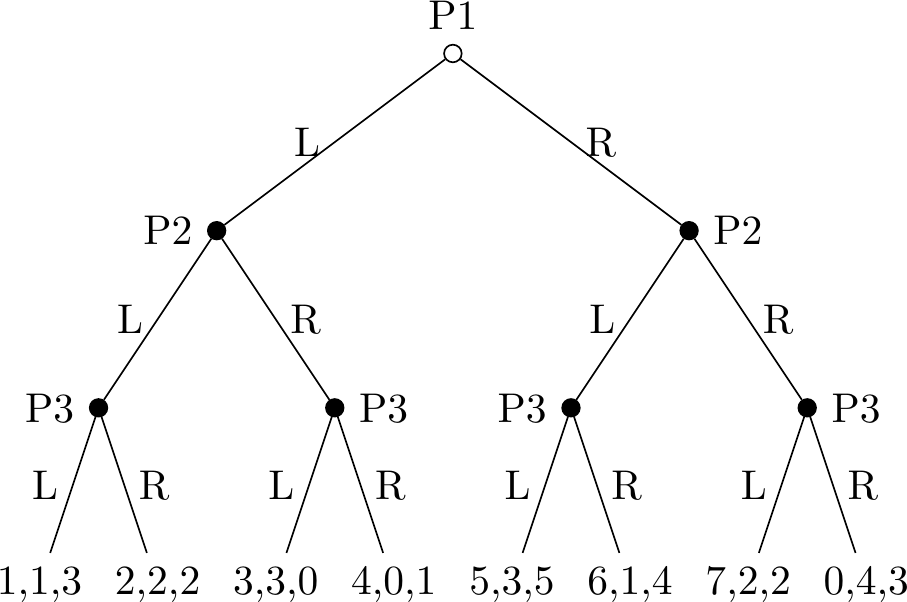
\includegraphics{sample_exam_files/figure-pdf/fig-back-1.png}

}

\caption{\label{fig-back}Tree for Q10}

\end{figure}%

\begin{figure}

\centering{

\includegraphics{sample_exam_files/figure-pdf/fig-signal-1.png}

}

\caption{\label{fig-signal}Tree for Q11}

\end{figure}%



\end{document}
